\section{Artificial Intelligence}
As mentioned earlier, there is no scripting language in \doom. The A.I is based on a per enemy type state machine which is baked inside the engine binary. Designers did not have to learn C since they could entirely configure an opponent via a text file \cw{multigen.txt}. This text file is parsed by a tool (cunningly named \cw{multigen}) and compiled into a C structure (\cw{info.h} and \cw{info.c}).\\
\par
\rawdrawing{multigen}
\par
% The script has two sections per entity. First the general info and then a serie of state machines. To illustrate here if the imp script.\\
Let's dive into the step machine descriptor text file right away and take a look at the section of \cw{multigen.txt}  which describe the Imp (known as \cw{TROOP} internally).\\
\par
\tcode{enemy_info.txt}

\tcode{imp_state.txt}

There are four sections. Properties such as DoomED \cw{id}, \cw{speed}, \cw{height}, \cw{radius}. State names for state machine targets. Sound strings. And finally the huge Action definition.






Properties list and sound names are self-explanatory, no need to spend too much time on it. What is more difficult to understand is how the state machine is defined.\\
\par
A thing state machine is partly statically defined inside the engine (when a monster is attacked it goes directly to \cw{seestate}, when it receive lethal damage, it does direcly to \cw{diestate}) and partly defined in \cw{multigen.txt}. Each line is the state definition follows a syntax.
\begin{enumerate}
\item State name.
\item Frame family.
\item Frame ID (sprite to render).
\item Duration in tics (engine runs 35 tics/seconds).
\item Function to call when in this state.
\item Next state.
\end{enumerate}
\par
Let's take the example of an Imp which was just spawned in a level and therefore is in state \cw{spawnstate} which is \cw{S\_TROO\_STND}. Upon simulating each game tic, the engine looks at what to do in this state. In this case, the Imp will cycle between state action \cw{S\_TROO\_STND} and \cw{S\_TROO\_STND2}. In these sub-states, \cw{A\_Look} is called each tics trying to detect the player. If it does, the engine place the imp in \cw{seestate} (a.k.a S\_TROO\_RUN1)\\
\par

Now this Imp was unlucky, the player was fast and managed to hit it with a shotgun at point blank. In this case the engine place the Imp in the Imp's \cw{deathstate} (\cw{S\_TROO\_DIE1}).\\
\par
\tcode{enemy_state_die.txt}\\
\par
Notice how values \cw{I}, \cw{J}, \cw{K}, \cw{L}, and \cw{M} are translated to sprite names.\\
\par
\fullimage{imp_die}
\par


\pagebreak
Let's follow the chain of state from here, where an imp dies in five steps.

\begin{enumerate}
\item Show first death frame (I) for 8/35th of a second.
\item Show second death frame (J) for 8/35th of a second. Scream using \cw{deathsound}.
\item Show third death frame (K) for 6/35th of a second.
\item Show fourth death frame (L) for 6/35th of a second. Mark itself as non-obstacle (\cw{A\_FALL}).
\item Show fifth death frame (M) forever (\cw{-1}).
\end{enumerate}
\par
The total dying sequence lasts $8+8+6+6=24/35 = 0.68$ second. Note that this Imp could have been even less lucky and been hit by a rocket. Enough damage would have gibbed it into \cw{xdeathstate} (\cw{S\_TROO\_XDIE1}) state and made it die in $1$ second.\\
\par
\tcode{enemy_state_xdie.txt}\\
\par
\fullimage{imp_xdie}




\par
\begin{wrapfigure}[9]{r}{0.25\textwidth}
\centering

\includegraphics[width=.25\textwidth]{drawings/sprite_quantization.pdf}
\end{wrapfigure}
The engine uses a convention to find what sprite to use when rendering them. Because an enemy will not always be facing the player, it uses quantization where all orientation with regard to the player position fall into eight buckets (see drawing where 1 is facing player, 5 back to player and so on).\\
\par
When in \cw{S\_TROO\_XDIE1} state, according to \cw{multigen.txt}, the engine must use sprite family \cw{TROO} and frame \cw{N}. Based on the orientation (lets say the Imp is back to the player), the engine should use \cw{TROON5}. But since these is no such sprite in \cw{DOOM.WAD} (exploding enemies always face the player) the engine falls back to \cw{TROONO} (0 being the "always facing" sprite).
\par







\cfullimage{cyber_sprite}{CyberDemon poses in one of its two "walk" position}
\par
Taking a look at one of the frame for the Cyberdemon in figure \ref{cyber_sprite} give a good idea of the colossal work required from artists. Twelve monsters times eight states times average of five frames per animation would have required close to 480 drawings (for the monsters only). The power of the NextDimension made a tremendous different in this department.\\
\par
The cyberdemon however is an extreme case since it is not symmetric. Imps sprite storage is optimized to take advantage of its symmetry. If the engine needs \cw{TROOA6} but doesn't find it in the \cw{WAD}, it uses its opposite (\cw{TROOA4}) and draws it horizontally inverted.\\ 
\par
\trivia{You may have noticed in the list of state, a non obvious one named \cw{RAISE}. It is used when the Arch-vile enemy resurrects a dead monsters. The animation plays the dying frame in reverse. Not that there are no reverse gibing so Arch-vile doesn't revive gibbed monsters.}




\begin{figure}[H] \centering
\cscaledimage{0.9}{imp_sprite}{}
\end{figure}
\par
\trivia{When an entity receives more than  \cw{spawnhealth} damage (negative its spawing state, in the case of an imp that would be -60), the engine triggers not \cw{deathstate} but \cw{xdeathstate} state which means the entity exploded.}\\
\par 
\ccode{explode.c}





\cw{multigen.txt} is compiled to an humongous 5000 lines \cw{info.c} made of an array of \cw{state\_t} holding the state machine and an array of \cw{mobjinfo\_t} holding the things properties.\\
\par
\ccode{enemy_state_compiled.c}\\
\par
\begin{wrapfigure}[9]{r}{0.5\textwidth}
\centering
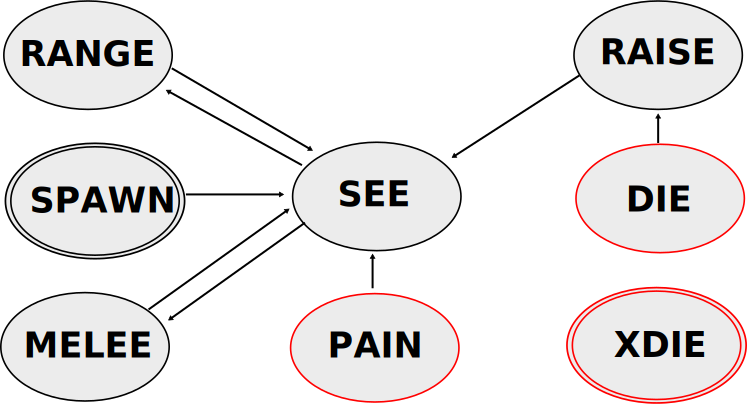
\includegraphics[width=.5\textwidth]{drawings/automate.pdf}
\end{wrapfigure}
Not all automaton state changes can be inferred from the transition array. In the case of the Imp, transitions are partly dictated by the logic in \cw{info.txt} (black arrows) and partly dictated by the game engine.\\
\par
 In the state diagram, engine triggered transitions to \cw{pain}, \cw{die}, and \cw{xdie} are not represented since these states can be reached directivity from any other state.
\par
%In the diagram, note the starting state (\cw{SPAWN}) and the only final state \cw{XDIE}. \cw{DIE} can transition to \cw{RAISE} thanks to the Archville heal power which makes the dead rise. The only way to make sure a monster will never come back is to gib it.

\pagebreak

\subsection{Optimization}
All monsters in a level are initialized in the \cw{spawnstate} which usually involves cycling a two frames animation (monsters do no have stand script, they "walk still") and calling \cw{A\_Look} method to attempt to see the player. Looking for the player constantly proved to be an unacceptable level of load on the CPU. Even using the blockmap structure to speed up collision detection it still meant hundreds of rays to cast, twenty five times per second which resulted in thousand and thousand of instructions.\\
\par
To solve this problem, an other datastructre was introduced with \cw{doombsp}. For each sectors, a potentially visible sector bit array is calculated\footnote{This approach later morphed into the Potentially Visible Set which was instrumental to Quake engine.}. This dataset is packed into a matrix of size $num\_sectors^2/8$ and stored in a \cw{REJECT} lump. At runtime, the engine just compares the player's current sector with a monster's sector to potentially bypass collision detections for this monster entirely.\\
\par
\drawing{reject_explained}{}
% Regardless of the monsters, the base state machine looks like this but it tuned based on custom functions called in some states (e.g: \cw{A\_SpidRefire}, \cw{A\_CyberAttack}, and \cw{A\_BrainExplode}).\\
% \par
% \pngdrawing{automate}{}
Figure \ref{reject_explained} features three sectors with five monsters and one player. The engine needs only to run one monster I.A seeking for the player since the later is in sector \circled{1}. All four others monsters are "rejected" until the player most inside sector \circled{3}. The table is only used for sight. Monsters will still hear the player since sound is cheaper to propagate.\\
\par
\trivia{With "unlimited" CPU power, modern Node Builder don't build \cw{REJECT} anymore.}






\section{Map Intelligence}
Despite lacking a scripting system, maps still managed to offer a rich experience. They were full of surprises with numerous elements interacting with the player. Switches and tripwire-enabled doors, secret passages, elevators, crushing walls, traps and many others.\\
\par
\pngdrawing{tripwire}{E1M1 features \color{red}{XX} special lines + IMAGE ABOVE TODO}
\par
All interactions are achieved via a simple association between a line's \cw{special} attribute which designates one action to perform and one \cw{tag} value which is the target sector to act on.\\
\par
The list of types of actions is impressive, there are more than 130 of them. Open/Close door at normal/turbo/blazing speeds. Raise/Lower floor and ceilings, Fast Ceiling Crush \& Raise, Build Stairs, Lock door so you are trapped with monsters, Change light levels, Raise floor to nearest height, change texture, teleport, Exit level, Secret exit, and many others.\\
\par
The tag designating the target is any number picked by the designed. Any lines the designer wants to be targeted by this action is tagged with the same number. With this system, a line can trigger only one action but target several sectors.\\
\par
\trivia{No doubt the countless hours the team spent playing Dungeons \& Dragons came handy when it came to design \doom's mazes.}
\pagebreak






\begin{wrapfigure}[17]{r}{0.5\textwidth}
\centering
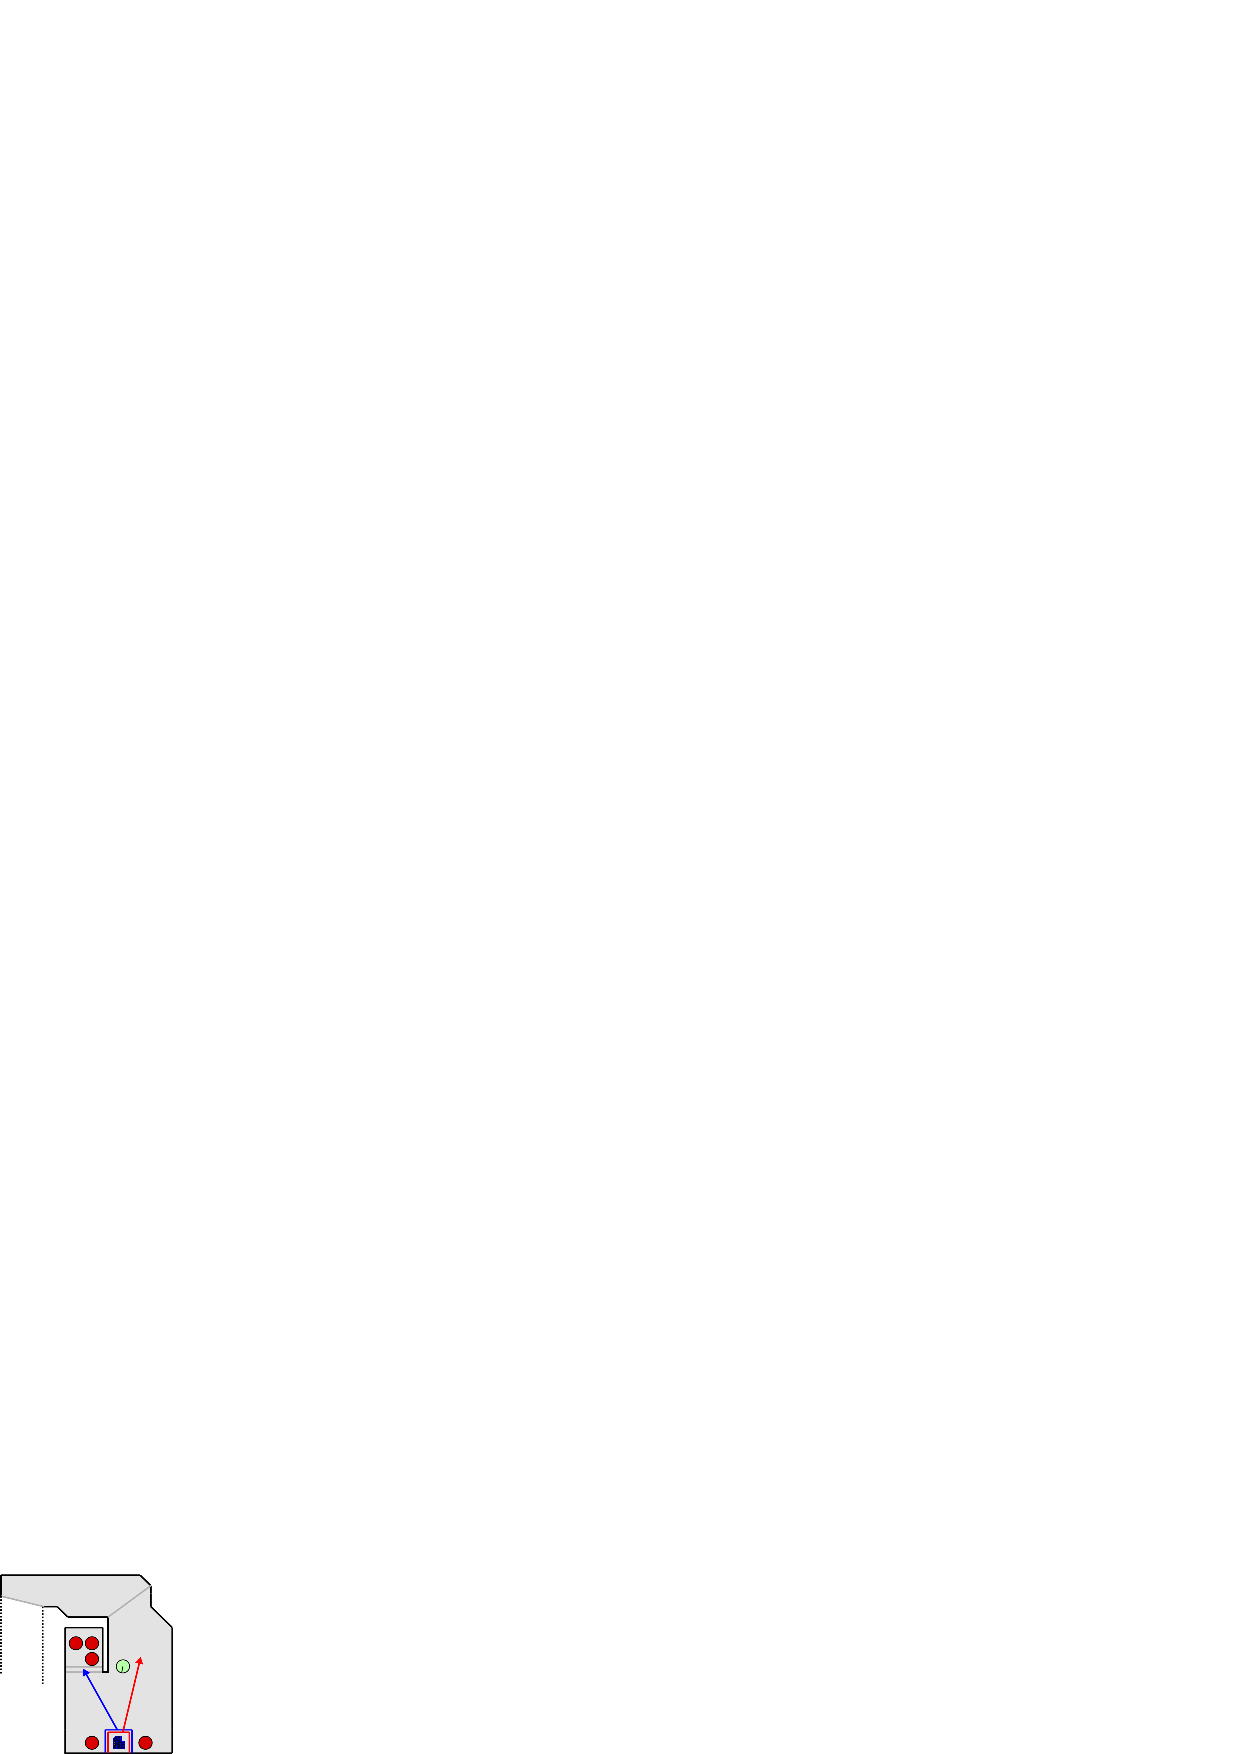
\includegraphics[width=.5\textwidth]{drawings/E1M3_trap.pdf}
\end{wrapfigure}
Who doesn't recognize E1M3 hunt for the blue key on page \pageref{e1m3_trap}. After traversing the whole map, it is finally there shining on a pedestral. Guarded by only two low levels opponents which are easily dispatched.\\
\par
But as soon as the player picks it up, all lights go off and the combined sound of a door opening and growling Imps leaves no doubt: It was trap doomguy just walked in and Imps are just behind him (page \pageref{e1m3_trap})!\\
\par
To implement this effects, two set of lines were used. The first lines (in blue) targets the door sector via tag YY where the monsters were hiding and opens it. The second lines (in red) targets the current sector via tag XX and set its light level to "very dark".\\
\par



\par
\begin{wrapfigure}[23]{l}{0.5\textwidth}
\centering
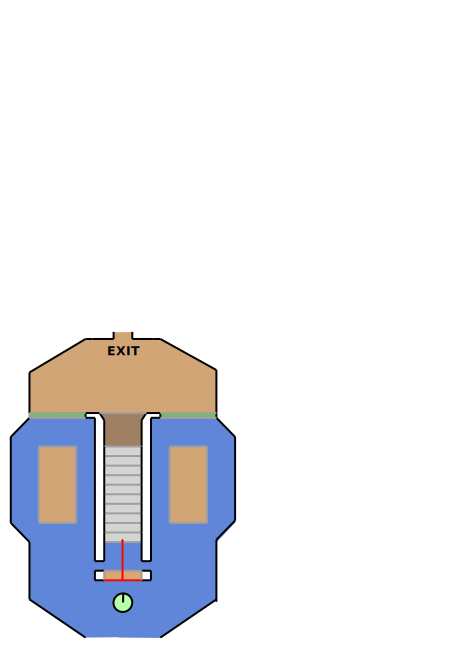
\includegraphics[width=.5\textwidth]{drawings/E1M3_sides2.pdf}
\end{wrapfigure}
An other interesting effect in E1M3 is the rising stair which leads to the small room containing the exit to level 4. It is implemented by having a line with special code "BuildStairs" (\#8) targeting the first step sector with its tag. The engine has a hardcoded \cw{EV\_BuildStairs} which looks up the target sector via the tag then uses a flood-fill algorithm.\\
\par Adjacent sectors are repeatedly looked up and a little bit of height is added each iteration. To avoid raising the whole level, the algorithm stops flowing when the next sector texture is different from the last elevated sector which explains why the stairs are grey while bottom and top are blue and brown.\\
\par
Before and after screenshots can be seen on page \pageref{stairs}.

\label{e1m3_trap}
\fullimage{Doom-E1M3-Ingame2.png}\\

Finally, the blue key (above)! Nooo, it's a TRAP (below)!

\vspace{2mm}
\fullimage{Doom-E1M3-Ingame3.png}


\fullimage{e1m3_after_stairs.png}\\

Above, all steps of the stairs are at the same level. Below, a line triggered "BuildStairs". \label{stairs}

\vspace{2mm}
\fullimage{e1m3_before_stairs.png}













\pagebreak
\section{Game tics Architecture}
With the knowledge of how opponents and map elements work, we can pickup the code where we had left it with regard to game simulation on page \pageref{TryRunTics.c}. \cw{G\_Ticker} is where all thinkers tic.\\
\par
\ccode{G_Ticker.c}
\par
Most of the meat is in the 3D gameplay (\cw{P\_Ticker}) function.\\
\par
\ccode{P_Ticker.c}
\par
\cw{P\_PlayerThink} is where player is allowed to "think". Namely where the \cw{cmd\_t} (which we already studied on page \pageref{cmd_t_type}) are consumed.\\
\par 
\cw{P\_RunThinkers} is how the map and monsters "think". Anything that must occur over more than one frame is placed in a thinker object and stored in a double linked list. Thinker are struct with a function pointer and some data for the function pointer parameters. Each gameplay tic, it let's every thinker in the list "think". Thinker which are done thinking set their function pointer to -1 so they are dropped from the list. Note that doors have no feelings but they are nonetheless "thinkers" too.\\
\par
\cw{P\_UpdateSpecials} takes care of animating special texture such as water, or living walls. It also takes care of switching the texture when a button is pushed.\\
\par 

 \cw{P\_RespawnSpecials} respawns medikits, weapons, and ammo in deathmatch.




\ccode{thinker_t.c}\\
\par
C has no OOP capabilities yet the engine managed to implement a polymorphism system. Semantically, \cw{think\_t} are stored in the linked list element (\cw{thinker\_t}) with no space for the payload. \\%But since all thinkers start with a function pointer, the engine stores the function pointer and the data parameter payload with a single pointer. \\
\par
\ccode{floormove_t.c}\\
\par
\cw{EV\_BuildStairs} which creates a thinker to elevate floors, shows how to use the system.\\
\par
\ccode{EV_BuildStairs.c}\\
\par
For this thinker, what ends up being called during a game tic is \cw{floor->thinker(floor)}.
